	\chapter{Statistics}
	\formattedepigraph{All models are wrong, but some models are useful.}{George Box}

The five characteristic numbers:
	\begin{plainlist}
		\item \xsmallest{}
		\item \quartileone{}
		\item \quartiletwo{}
		\item \quartilethree{}
		\item \xlargest{}
	\end{plainlist}

Box plot, maximum 1.5 times interquartile range below the first quartile or above the third quartile.  The rest are outliers and plot them accordingly.



median formula?
	\begin{eqnarray}
		\variance 					& = & \frac{1}{N-1}\sum^N_{i=1}\left(x_i - \samplemean\right)^2 \\
		\samplestandarddeviation	& = & \sqrt{\variance}
	\end{eqnarray}
Note that this version assumes equal probability of all data.



coefficient of variation

	\begin{figure}[tbp]
		\centering
		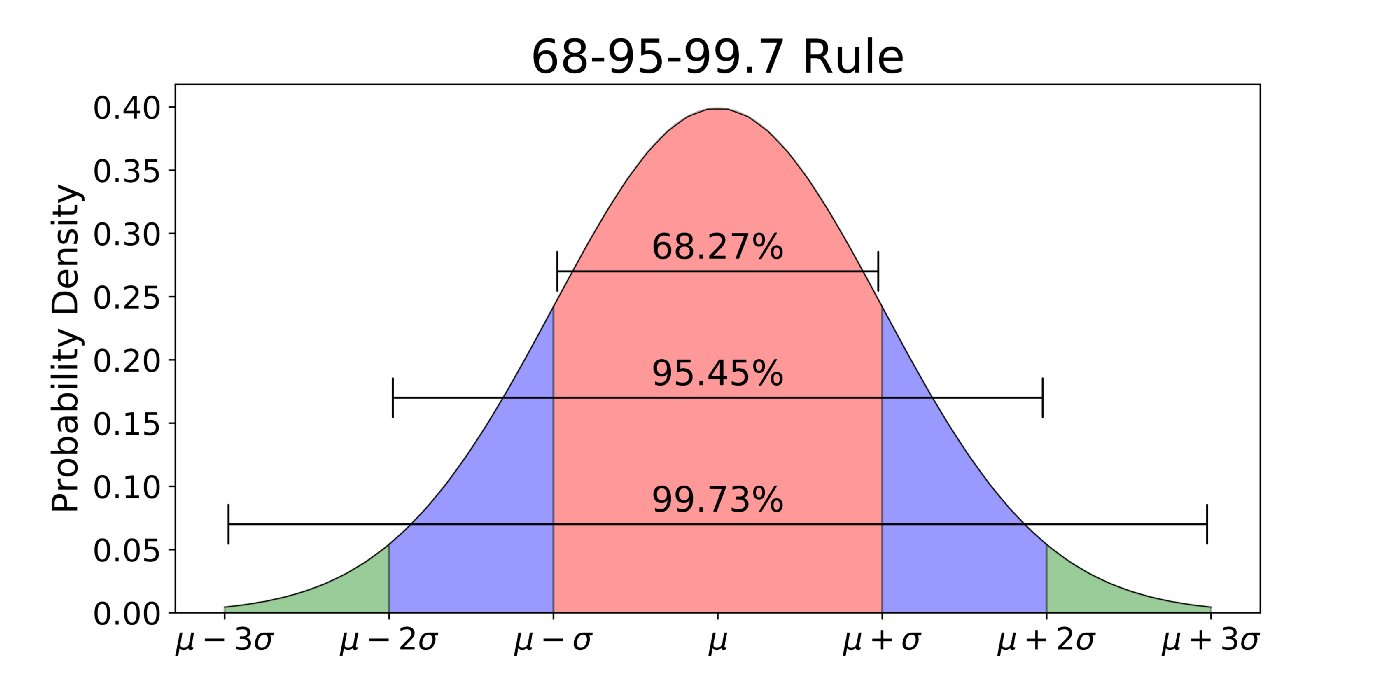
\includegraphics[height=2.5in]{normaldistrution}
		\caption[Normal distribution]{Normal distribution.}
		\label{fig:normaldistrution}
	\end{figure}

The normal distribution is characterized by two parameters, the mean (\populationmean) and the standard deviation (\populationstandarddeviation).

	\section{Z-Score}
The Z-score is a measure the number of standard deviations away from the mean that a data point is.

	\subsection{One Sample Formula}
To get the Z-score of a variable, subtract the mean and divide by the standard deviation:
	\begin{equation}
		Z = \frac{X-\populationmean}{\populationstandarddeviation}
	\end{equation}
	\begin{mathwhere}
		\mathdefitem{X}{the observed data point.}
	\end{mathwhere}

	\subsection{Multiple Sample Formula}
When you have multiple samples and want to describe the standard deviation of the sample's mean, the z-score formula substitutes the standard deviation error estimation for the standard deviation.  See \sectionname~\ref{sec:errorestimation} for more information.
	\begin{equation}
		Z = \frac{X-\populationmean}{\frac{\populationstandarddeviation}{\sqrt{n}}	}
	\end{equation}

	\section{Error Estimation}
	\label{sec:errorestimation}
When the mean (or other value) is calculated from the sample, it is not the mean of the population.  We want to know the accuracy of that estimated value.  We express that accuracy as a confidence interval.  We do that by calculating the error and then
	\begin{eqnarray}
		E = \frac{\populationstandarddeviation}{\sqrt{n}}	& \quad\quad & \text{error estimate}	\\
		\samplemean - E								& 		& \text{lower error bound}				\\
		\samplemean + E								& 		& \text{upper error bound}
	\end{eqnarray}
	\begin{mathwhere}[0.38in]
		\mathdefitem{E}{error estimate;}
		\mathdefitem{\populationstandarddeviation}{population standard deviation;}
		\mathdefitem{n}{number of sample points used to calculate the sample value (mean, et cetera);}
		\mathdefitem{\samplemean}{sample mean.}
	\end{mathwhere}
For more on this, see \sectionname~\ref{sec:centrallimittheorem}

	\section{Central Limit Theorem}
	\label{sec:centrallimittheorem}
The standard deviation of \samplemean{}, also called the ``standard error of \samplemean{}'' is:
	\begin{equation}
		\frac{\populationmean}{\sqrt{n}}
	\end{equation}
	\begin{mathwhere}
		\mathdefitem{n}{the sample size.}
	\end{mathwhere}
This holds even if the population is not normally distributed.  As the sample size gets bigger, the sample means will approach a normal distribution no matter what the shape of the population distribution is.  This is known as the \textit{Central Limit Theorem}.

The \textit{Central Limit Theorem} assumes:
	\begin{bulletedlist}
		\item Data is randomly sampled.
		\item Sample values are independent of each other.
		\item Samples are from the same distribution.
		\item Sample size is sufficiently large.
	\end{bulletedlist}


	\section{Binomial Distribution}
The probability function of a Binomial Distribution provides the probability for $x$ number of successes from $n$ trials as
	\begin{equation}
		P(X=x) = \binom{n}{x}p^x\left(1-p\right)^{n-x}
	\end{equation}
	\begin{mathwhere}
		\mathdefitem{P}{total probability of $x$ successes from $n$ trials;}
		\mathdefitem{x}{number of successes;}
		\mathdefitem{n}{number of trials;}
		\mathdefitem{p}{probability of success of an individual trial.}
	\end{mathwhere}


	\section{Uniform Distribution}
	\begin{displaymath}
		U\left(a, b\right)
	\end{displaymath}
	\begin{displaymath}
		U\left[a, b\right]
	\end{displaymath}
Uniform distribution:
	\begin{mathwhere}[0.38in]
		\mathdefitem{\left(, \right)}{open uniform distribution over the range of $a$ and $b$;}
		\mathdefitem{\left[, \right]}{closed uniform distribution over the range of $a$ and $b$;}
		\mathdefitem{a}{Lower bound;}
		\mathdefitem{b}{Upper bound;}
	\end{mathwhere}

	\section{Student's T-Distribution}
Student's t-distribution is a family of continuous probability distributions that arise when estimating the mean of a normally distributed population in situations where the sample size is small and the population's standard deviation is unknown (\referencename~\cite{ref:wikipediatdistribution}).

	\begin{bulletedlist}
		\item Continuous data.
		\item Normally distributed.
		\item Small sample size.
		\item Unknown population standard deviation.
		\item Random sampling from the population.
	\end{bulletedlist}

	\section{Analysis of Variance (\acrshort{anova})}
Response: Dependent variable which is continuous and assumed to follow a normal distribution.
Factor: Independent explanatory variable with several levels.
Number of factors: How many variables are used.

	\begin{equation}
		\textrm{f-statistic} = \frac{\textrm{between group variations}}{\textrm{within group variations}}
	\end{equation}
A large f-statistic indicates there is more variation between groups than within groups.  Thus, it will provide evidence against the null hypothesis.

One-way \acrshort{anova}

	\begin{figure}[tbp]
		\centering
		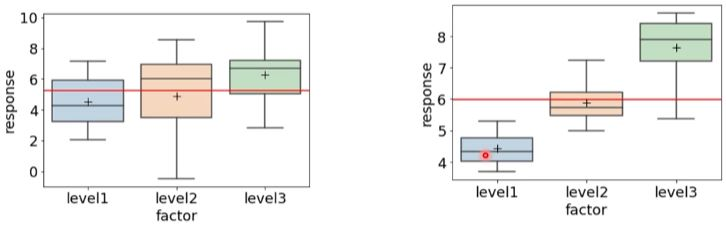
\includegraphics[height=1.75in]{anovalevelversusfactor}
		\caption[Levels versus factors for ANOVA]{Levels versus factors for \acrshort{anova}.}
		\label{fig:anovalevelversusfactor}
	\end{figure}

	\section{Hypothesis Testing}
Type 1 error (false positive): Concluding there is a change in probability when there is not.  The null hypothesis is true, but it is rejected.  Probability of a Type 1 error is denoted as \levelofsignificance{}.

Type 2 error (false negative): Concluding there is not a change in probability when there is.

	\begin{figure}[tbp]
		\centering
		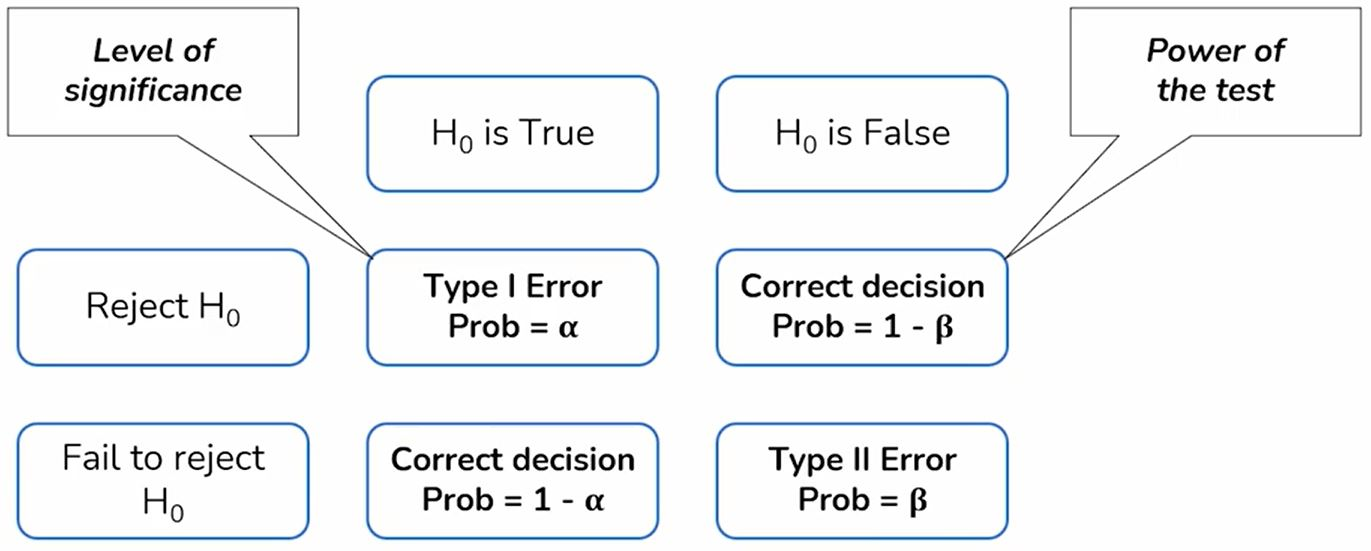
\includegraphics[height=2.5in]{type1andtype2errors}
		\caption[Hypothesis testing errors]{Hypothesis testing errors.}
		\label{fig:type1andtype2errors}
	\end{figure}

	\begin{numberedlist}
		\item Identify the key questions.
		\item Establish the hypotheses.
		\item Understand and prepare data.
		\item Identify the right test.
		\item Check the assumptions.
		\item Perform the test.
	\end{numberedlist}

	\begin{figure}[tbp]
		\centering
		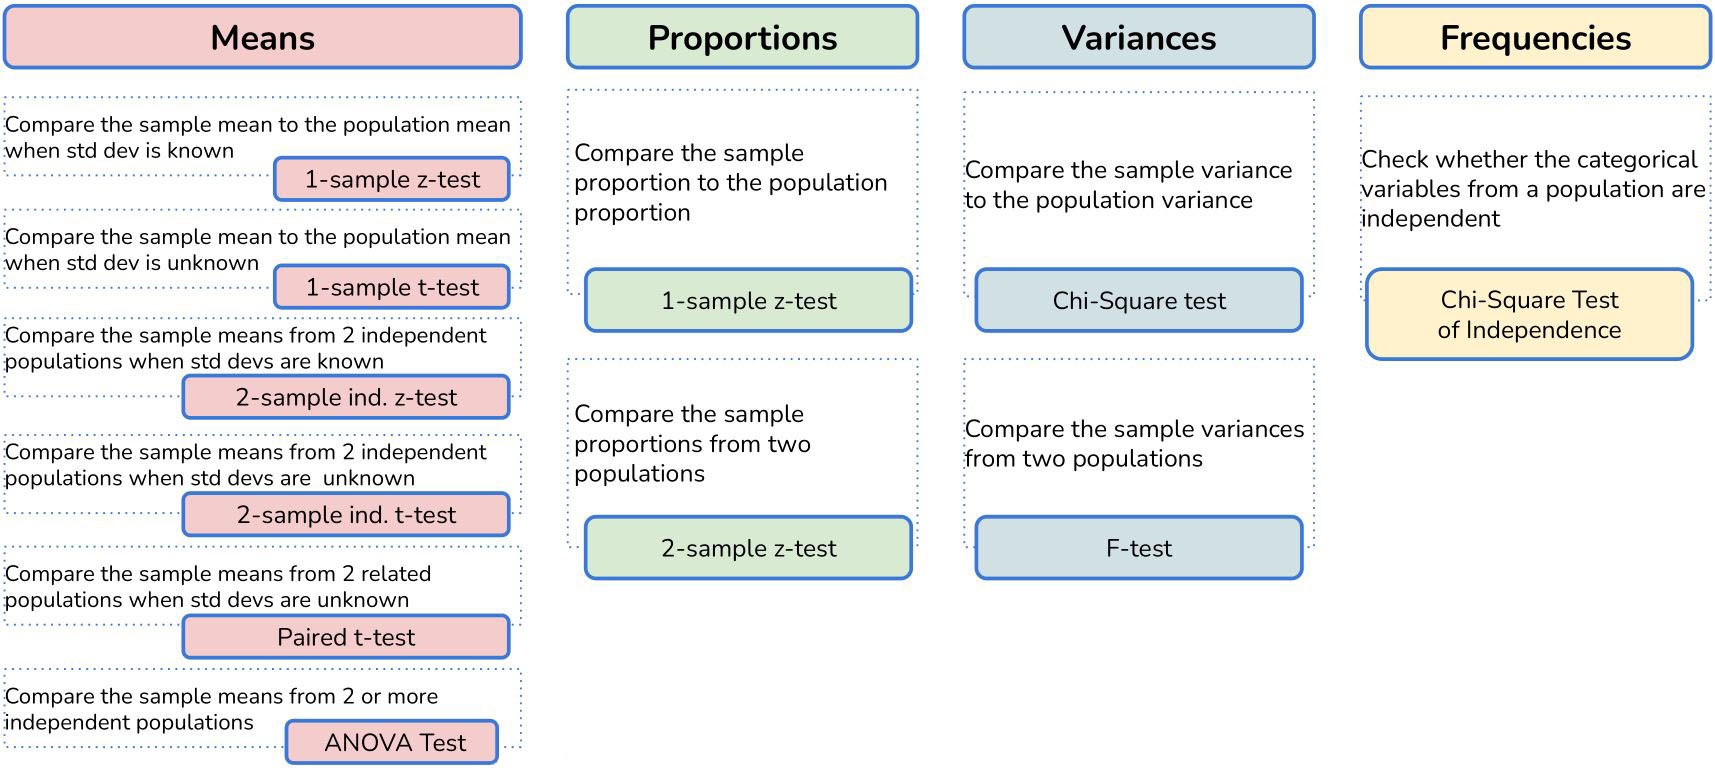
\includegraphics[width=6.0in]{hypothesistests}
		\caption[Hypothesis test matrix]{Hypothesis test matrix.}
		\label{fig:hypothesistests}
	\end{figure}

	\begin{figure}[tbp]
		\centering
		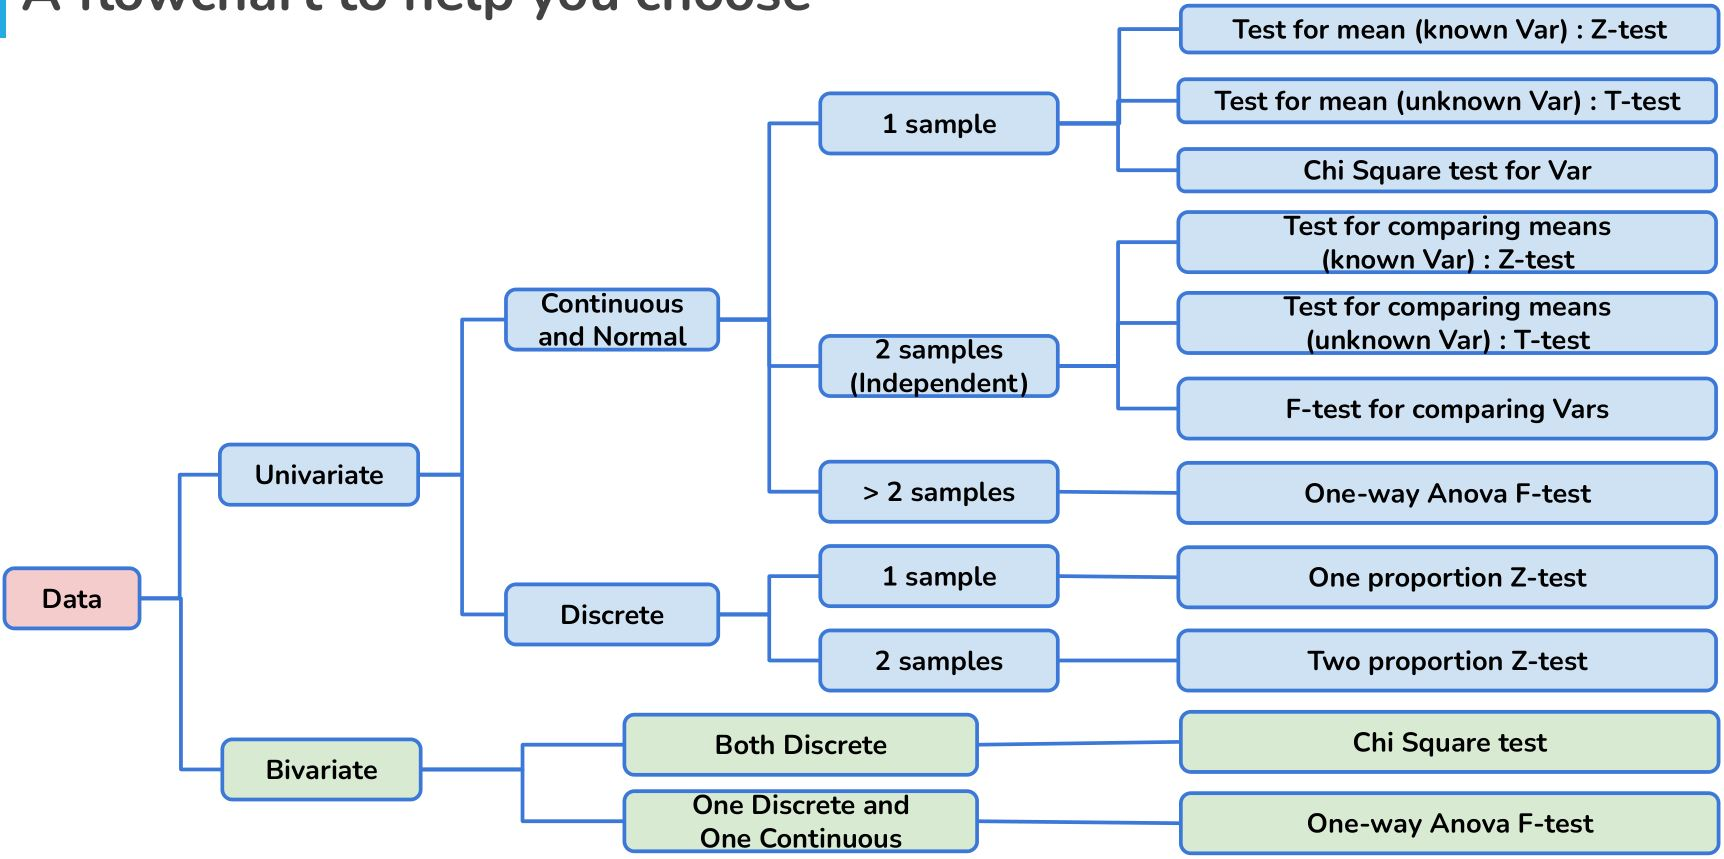
\includegraphics[width=6.0in]{hypothesistestflowchart}
		\caption[Hypothesis test flow chart]{Hypothesis test flow chart.}
		\label{fig:hypothesistestflowchart}
	\end{figure}



\newpage{}
%    \begin{table}
%        \centering
%        \caption{Comparison of Hypothesis Test Types.  See the Jupiter notebook "Hypothesis Testing Statistical Learning Week 2" for more information and examples.}
%        \label{tab:hypothesistests}
% \tabledoublecline{1}{4}
        \begin{longtable}{|N|p{1.25in}|p{3.08in}|p{1.2in}|}
        	\caption[Comparison of hypothesis test types]{Comparison of hypothesis test types.  See the Jupiter notebook ``Hypothesis Testing Statistical Learning Week 2'' for more information and examples.}
         	\label{tab:comparisonofhypothesistesttypes}\\
        	\hline
			\multicolumn{1}{|c|}{} & \tablecolumnheadervlinestwo{Significance of Test} &
				\tablecolumnheadervlinestwo{Assumptions} &
				\tablecolumnheadervlinestwo{Distribution/Test} \endhead \hline
			\label{trw:populationmean} &
				Population mean $\nullhypothesis : \populationmean = \populationmean_0$ &
				\begin{nospacebulletedlist}
					\item Continuous data
					\item Normally distributed
					\item Sample size \textless{}30
					\item Random sampling
					\item Unknown population standard deviation
				\end{nospacebulletedlist} &
				\distributiontest{t-distribution}{one sample t-test} \\ \hline
			\label{trw:twopopulationmeans} &
				Equality of two population means \newline$\nullhypothesis : \populationmean_1 = \populationmean_2$ &
				\begin{nospacebulletedlist}
					\item Continuous data
					\item Normally distributed or sample size \textgreater{}30
					\item Independent populations
					\item Random sampling
					\item Known population standard deviations
				\end{nospacebulletedlist} &
				\distributiontest{normal distribution}{two independent sample z-test} \\ \hline
			\label{trw:equalityofmeansequalunknownstandarddeviation} &
				Equality of means with equal and unknown standard deviation \newline$\nullhypothesis : \populationmean_1 = \populationmean_2$ &
				\begin{nospacebulletedlist}
					\item Continuous data
					\item Normally distributed
					\item Independent populations
					\item Random sampling
					\item Equal population standard deviations
				\end{nospacebulletedlist} &
				\distributiontest{t-distribution}{two independent sample t-test} \\ \hline
			\label{trw:equalityofmeansunequalunknownstandarddeviation} &
				Equality of means with unequal and unknown standard deviations \newline$\nullhypothesis : \populationmean_1 = \populationmean_2$ &
				\begin{nospacebulletedlist}
					\item Continuous data
					\item Normally distributed
					\item Independent populations
					\item Random sampling
					\item Unequal population standard deviations
				\end{nospacebulletedlist} &
				\distributiontest{t-distribution}{two independent sample t-test} \\ \hline
			\label{trw:pairedpoints} &
				Equality of two population means when sample points are paired \newline$\nullhypothesis : \populationmean_1 = \populationmean_2$ \vspace*{1pt} &
				\begin{nospacebulletedlist}
					\item Continuous data
					\item Normally distributed
					\item Independent populations
					\item Random sampling
				\end{nospacebulletedlist} &
				\distributiontest{t-distribution}{paired t-test} \\ \hline
			\label{trw:oneproportion} &
				Population proportion \newline$\nullhypothesis : \proportion = \proportion_0$ &
				\begin{nospacebulletedlist}
					\item Binomial distribution
					\item Random sampling
					\item When both mean (np) and n(1-p) are greater than or equal to 10, the binomial distribution can be approximated by a normal distribution
				\end{nospacebulletedlist} &
				\distributiontest{normal distribution}{one proportion z-test} \\ \hline
			\label{trw:equalityoftwoproportions} &
				Equality of two population proportions \newline$\nullhypothesis : \proportion_1 = \proportion_2 $ &
				\begin{nospacebulletedlist}
					\item Binomial distribution
					\item Independent populations
					\item Random sampling
					\item When both mean (np) and n(1-p) are greater than or equal to 10, the binomial distribution can be approximated by a normal distribution
				\end{nospacebulletedlist} &
				\distributiontest{normal distribution}{two proportion z-test} \\ \hline
			\label{trw:onevariance} &
				Population variance \newline$\nullhypothesis : \populationvariance = \populationvariance_0$ &
				\begin{nospacebulletedlist}
					\item Continuous data
					\item Normally distributed
					\item Random sampling
				\end{nospacebulletedlist} &
				\distributiontest{chi-square distribution}{chi-square test for variance} \vspace*{2pt} \\ \hline
			\label{trw:equalityofvariances} &
				Equality of two population variances \newline$\nullhypothesis : \populationvariance_1 = \populationvariance_2$ &
				\begin{nospacebulletedlist}
					\item Normally distributed
					\item Independent populations
					\item Larger variance should be placed in the numerator
				\end{nospacebulletedlist} &
				\distributiontest{F-distribution}{F-test for variances} \\ \hline
			\label{trw:chisquaredindependence} &
				In a contingency tables \newline$\nullhypothesis : $ The row and column variables are independent \vspace*{1pt} &
				\begin{nospacebulletedlist}
					\item Random sampling
					\item Categorical variables
					\item Expected value of the number of sample observations in each level of the variable is at least 5
				\end{nospacebulletedlist} &
				\distributiontest{chi-squared distribution}{chi-squared test of independence} \\ \hline
			\label{trw:anova} &
				Means for more than two populations \newline$\nullhypothesis : \populationmean_1 = \populationmean_2 = \arguments = \populationmean_n$ \vspace*{1pt} &
				\begin{nospacebulletedlist}
					\item Normally distributed
					\item Samples are independent simple random samples
					\item Populations variances are equal
				\end{nospacebulletedlist} &
				\distributiontest{F-distribution}{One-way \acrshort{anova} F-test} \\ \hline
        \end{longtable}
%    \end{table}


%			\label{trw:} &
%				\newline$\nullhypothesis : $ &
%				\begin{nospacebulletedlist}
%					\item
%				\end{nospacebulletedlist} &
%				\distributiontest{}{} \\ \hline

	\begin{code}{}
		\codeitem \ref{trw:populationmean}) scipy.stats.ttest\_1samp(\arguments)
		\codeitem \ref{trw:twopopulationmeans}) DistributionTests.TwoSampleZTest(\arguments)
		\codeitem \ref{trw:equalityofmeansequalunknownstandarddeviation}) scipy.stats.ttest\_ind(equal\_var=True, \arguments)
		\codeitem \ref{trw:equalityofmeansunequalunknownstandarddeviation}) scipy.stats.ttest\_ind(equal\_var=False, \arguments)
		\codeitem \ref{trw:pairedpoints}) scipy.stats.ttest\_rel(\arguments)
		\codeitem \ref{trw:oneproportion}) statsmodels.stats.proportion.proportions\_ztest([ints])
		\codeitem \ref{trw:equalityoftwoproportions}) statsmodels.stats.proportion.proportions\_ztest([numpy arrays])
		\codeitem \ref{trw:onevariance}) DistributionTests.ChiSquareVariance(\arguments)
		\codeitem \ref{trw:chisquaredindependence}) scipy.stats.chi2\_contingency(\arguments)
		\codeitem \ref{trw:anova}) scipy.stats.f\_oneway(\arguments)
	\end{code} 